\chapter{\leavevmode Introduction}
\label{chap:introduction}

% \section*{Overview}
% \addcontentsline{toc}{section}{Overview}
\section{Background}  \label{background}

Serial printers are devices commonly used for instant reporting of system data for industrial control systems (ICS) and receipts for point-of-sale (POS) systems. These devices are connected to their host using Wi-Fi, bluetooth, ethernet, or USB; in some cases, serial RS232 is an option as well. The goal of this research is to assess what software and hardware protections are enabled, as well as, how configurable the serial printers are for further exploit research.


\begin{figure}[ht]%
  \centering
  \subfloat[\centering Square POS]{{ 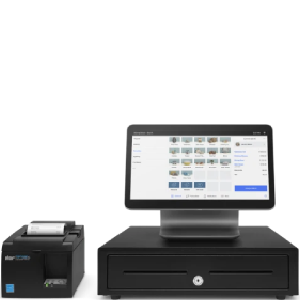
\includegraphics[width=0.30\textwidth,keepaspectratio]{Figures/MidSquare.png} }}%
  \qquad
  \subfloat[\centering SurePOS]{{ 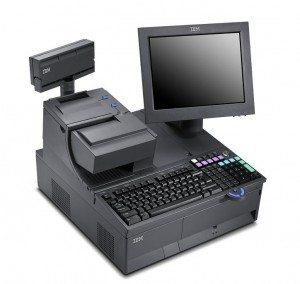
\includegraphics[width=0.25\textwidth,keepaspectratio]{Figures/SurePOS.jpg} }}%
  \caption{Comparison of common POS systems}%
  \label{fig:comparison_pos}%
\end{figure}

Figure \ref{fig:comparison_pos} shows us two similar looking point-of-sale systems. However, the operating system and required hardware used by both is different. Typically, unless you have the Square provided terminal, their software/client is installed onto an Android or iOS device and connected to a Square compatible card reader \autocite{ondrusMobilePaymentsMarket2011}. Whereas, the SurePoS, NCR, or other common EFTPoS system will run a proprietary OS based on Windows or Linux \autocite{ebimoboweiROLESOFTWARECASHLESS2018}. Furthermore, these PoS require some form of printing receipts as record keeping for the business owner and customer. And these devices also vary in terms of processing capabilities and operating system.

For instance, a common thermal printer seen with PoS systems, integrated with fuel pumps, or other industrial control equipment, is the SNBC BTP-S80 thermal printer \autocite{SNBCBTPS80Thermala,SNBCNewBeiyangIntelligent}. There are multiple versions of the device with support for Bluetooth, USB only, or combination of USB/Serial/Ethernet. The bluetooth hardware is provided over an accessory 25-pin serial connection, with more I/O as a serial connection via RS232C connector and USB Type-B. It has driver support for various platforms: Android, iOS, Windows, Linux, and MacOS. The most interesting aspects are the processor, an Arm Cortex M4 clocked at 3.54MHz, and the operating system, a proprietary version of FreeRTOS. The system architecture is Armv7E-M with JTAG/SWD hardware debugging support \autocite{CortexM4,FreeRTOSMarketLeading}.

By default, the printer has enough headroom to process ESC/POS commands for printing paper and a webserver for debugging or general diagnostics. In theory, the uncompromised device could be flashed with modified firmware to act as a decoy and human-input-device (HID) against the host PoS. The viability of any vulnerabilities would likely be dependent upon supply chain attacks or physical bait-and-switch tactics \autocite{scaifeFearReaperCharacterization2018}.

% In this paper, we propose exploring the processing capabilities and extensibility of FreeRTOS to act as a dual HID clone and printer for continued research.

\section{Significance}  \label{significance}

According to the Federal Trade Commission (FTC), there were 37,932 reports of credit card fraud in 2012 and 87,451 reports in 2022 \autocite{ConsumerSentinelNetwork2023,forthesentinelConsumerSentinelNetwork2022}. This marks an increase of credit card payment fraud by an estimated, 30.5\%. By comparison, since 2020, there has been a 14.6\% increase in credit card related fraud. Which does not include the millions of other fraud reports the FTC receives every year. In 2022 alone, there were around 5.1 million fraud, identity theft, and miscellaneous reports in total \autocite{ConsumerSentinelNetwork2023,forthesentinelConsumerSentinelNetwork2022}. The statistics for these reports stresses how crucial the security of payment systems are, both physical and online. And, the need to secure them grows every year.

Spyduino is \autocite{karystinosSpyduinoArduinoHID2019} a working example of a programmable BadUSB device using an Arduino to mimic a Human Interface Device (HID). Arduinos are typically more accessible and easily developed compared to an embedded device whose design is more single purpose \autocite{ComparativeStudyArduino,griffithsECIAIR2019European2019}. Especially if the goal is to not modify hardware or require hands-on access for exploitation. However, the research shows us that is it possible create HID clones from scratch if the hardware is compatible.

The Arduino used in their research is powered by an ATmega328P microcontroller with 32KB flash memory, 2KB SRAM, and 1KB EEPROM. Compared to the most likely target device of our proposed research, the SNBC BTP-S80, it features an ARM Cortex M4 microcontroller with 512KB flash memory, 96KB SRAM, 4KB of EEPROM. This is relevant to the proposed research, because it shows that a device with similar hardware specifications was feasible; meaning, it is likely that our own research will be successful. BadUSBs are a known and tested area of research. The novelty of this proposal comes from the assessment of the printer devices and showing whether one could be used maliciously within their environments (e.g., PoS systems, or ICS).

\section{Research Goals and Objectives}  \label{researchgoalsobjectives}

This research primarily focuses on physical POS systems or terminals and their hardware (serial accessories), rather than online solutions. For instance, not mobile payment apps like Venmo, CashApp, Zelle, or Paypal \autocite{wangMobilePaymentSecurity2016} since their environments typically do not use serial print devices. It is also likely that more research would be needed for emulating touch inputs for mobile environments versus the traditional keyboard attacks that will be implemented. Presumably, the host-to-guest communication will not differ greatly
between other environments (e.g., ICS). If the printers have demonstrable weaknesses with an Ubuntu host, that will fulfill the testing requirements.

The goal of this research is to further establish academic works in regards to embedded printer devices testing and security. This area is loosely documented within academia and only mentioned vaguely in relation to statistical reports or applied research using entirely different environments. For instance, most researchers limit their analysis of the environment to smartphones and the corresponding payment app, or detection systems for card skimmers \autocite{scaifeFearReaperCharacterization2018}.

Through this research we hope to identify supply chain risks using side channel attacks from auxiliary devices. Some examples of how the research could be applied in the future vary: BadUSB/BashBunny \autocite{hak5BashBunny}, JuiceShop \autocite{OWASPJuiceShop}, DVWA \autocite{woodDAMNVULNERABLEWEB2023}, or Webgoat \autocite{OWASPWebGoatOWASP}. Works within the PoS system context or embedded systems discussing supply chain attacks through third-party hardware are limited.

% \section{Printers}  \label{printers}

% \begin{figure}[ht]%
%   \centering
%   \subfloat[\centering BTP-S80]{{ 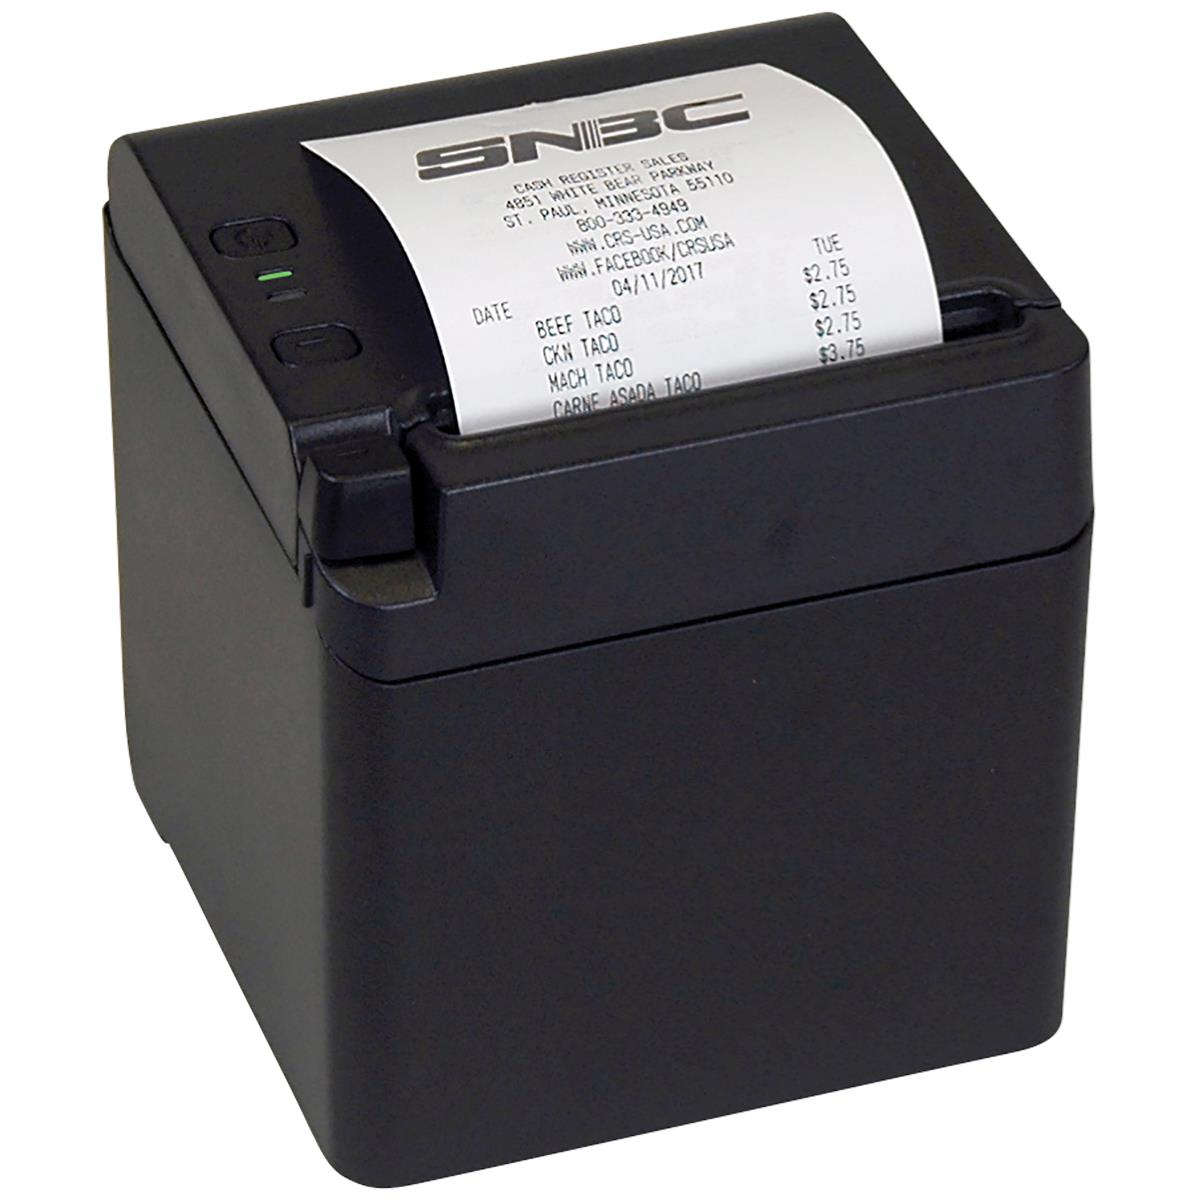
\includegraphics[width=0.40\textwidth,keepaspectratio]{Figures/SNBC_S80.jpeg} }}%
%   \qquad
%   \subfloat[\centering Printer I/O]{{ 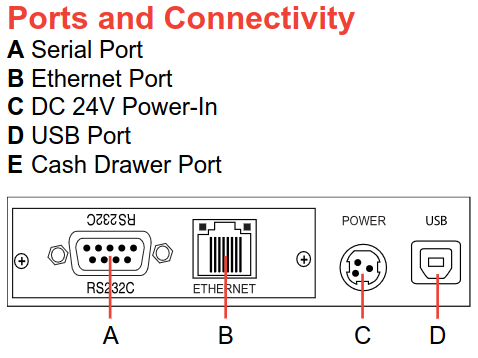
\includegraphics[width=0.40\textwidth,keepaspectratio]{Figures/SNBC_S80_IO.png} }}%
%   \caption{SNBC BTP-S80}%
%   \label{fig:btp_s80}%
% \end{figure}

% Figure \ref{fig:comparison_pos} shows us two similar looking point-of-sale systems, albeit one is much older looking. However, the operating system and required hardware is very different. Typically, unless you have the Square provided terminal, their software/client is installed onto an Android or iOS device and connected to a Square compatible card reader \autocite{ondrusMobilePaymentsMarket2011}. Whereas, the SurePoS, NCR, or other common EFTPoS system will run a proprietary OS derived from Windows or Linux \autocite{ebimoboweiROLESOFTWARECASHLESS2018}. Furthermore, these PoS tend to require some form of printing receipts as record keeping for the business owner and customer. And these devices also vary in terms of processing capabilities and operating system.

\section{Research Questions}  \label{researchquestions}

The research questions that this proposal seeks to answer are as follows:
\begin{itemize}
  \item Q1: Can the hardware be reflashed with a modified firmware image (e.g., FreeRTOS, ReconOS, VxWorks)? Testing a version of the original firmware with additional libraries, or an alternative OS, allows us to see if supply chain attacks are a concern. Either by the manufacturer, supplier, or other party. Reflashing is not novel by itself, however, the device might have protections in place to prevent it.  
  \item Q2: Does the hardware and firmware have enough resources to support HID functionality on-top of printing? In other words, can we maintain operation of standard printer command interpretation and side-channel input attacks without causing crashes or delays? The viability of the attack depends on it going unnoticed by operators or technicians. 
  \item Q3: Besides HID cloning, what other threat areas are exposed (e.g., network stack, web management portal, memory protections)? Are there any identifiable or known exploits when accessing the configuration panel (e.g., HTTP/2)? These provide a non-invasive method for bootstrapping the device.
\end{itemize}

Each of these goals will be approached individually as prescribed by the methodology.